\documentclass[border=2pt]{standalone}
\usepackage{amsmath,amssymb}
\usepackage{tikz}
\usetikzlibrary{positioning,arrows.meta,calc,fit}
\begin{document}
\footnotesize\hyphenpenalty=10000\exhyphenpenalty=10000
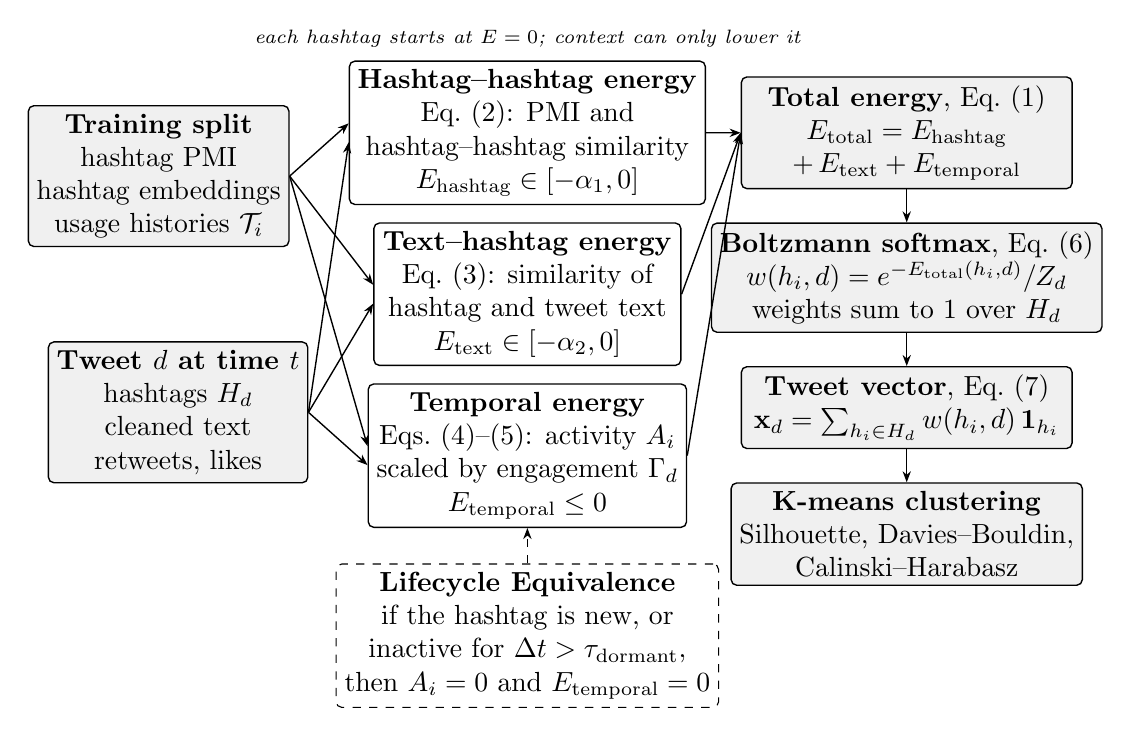
\begin{tikzpicture}[
  >={Stealth[length=4pt]},
  box/.style={draw, rounded corners=2pt, align=center, inner sep=3pt, line width=0.5pt},
  input/.style={box, fill=black!6, minimum width=2.8cm},
  energy/.style={box, fill=white, minimum width=3.9cm},
  stage/.style={box, fill=black!6, minimum width=4.2cm},
  rule/.style={draw, dashed, rounded corners=2pt, align=center, inner sep=3pt, minimum width=3.9cm, fill=white},
  lab/.style={font=\scriptsize\itshape, inner sep=1pt},
  arr/.style={->, line width=0.5pt},
]
% energies (middle column)
\node[energy] (eh) at (0,2.05) {\textbf{Hashtag--hashtag energy}\\ Eq.~(2): PMI and\\ hashtag--hashtag similarity\\ $E_{\text{hashtag}}\in[-\alpha_1,0]$};
\node[energy] (et) at (0,0) {\textbf{Text--hashtag energy}\\ Eq.~(3): similarity of\\ hashtag and tweet text\\ $E_{\text{text}}\in[-\alpha_2,0]$};
\node[energy] (ep) at (0,-2.05) {\textbf{Temporal energy}\\ Eqs.~(4)--(5): activity $A_i$\\ scaled by engagement $\Gamma_d$\\ $E_{\text{temporal}}\le 0$};
\node[rule, below=0.45cm of ep] (le) {\textbf{Lifecycle Equivalence}\\ if the hashtag is new, or\\ inactive for $\Delta t>\tau_{\text{dormant}}$,\\ then $A_i=0$ and $E_{\text{temporal}}=0$};
\draw[arr, dashed] (le) -- (ep);

% inputs (left column)
\node[input, left=0.75cm of eh, yshift=-0.55cm] (tr) {\textbf{Training split}\\ hashtag PMI\\ hashtag embeddings\\ usage histories $\mathcal{T}_i$};
\node[input, left=0.75cm of ep, yshift=0.55cm] (tw) {\textbf{Tweet $d$ at time $t$}\\ hashtags $H_d$\\ cleaned text\\ retweets, likes};

\foreach \e in {eh,et,ep} {
  \draw[arr] (tr.east) -- ($(\e.west)+(0,0.12)$);
  \draw[arr] (tw.east) -- ($(\e.west)+(0,-0.12)$);
}

% combination (right column)
\node[stage, right=0.75cm of et, yshift=2.05cm] (tot) {\textbf{Total energy}, Eq.~(1)\\ $E_{\text{total}}=E_{\text{hashtag}}$\\ $+\,E_{\text{text}}+E_{\text{temporal}}$};
\node[stage, below=0.42cm of tot] (sm) {\textbf{Boltzmann softmax}, Eq.~(6)\\ $w(h_i,d)=e^{-E_{\text{total}}(h_i,d)}/Z_d$\\ weights sum to 1 over $H_d$};
\node[stage, below=0.42cm of sm] (vec) {\textbf{Tweet vector}, Eq.~(7)\\ $\mathbf{x}_d=\sum_{h_i\in H_d} w(h_i,d)\,\mathbf{1}_{h_i}$};
\node[stage, below=0.42cm of vec] (km) {\textbf{K-means clustering}\\ Silhouette, Davies--Bouldin,\\ Calinski--Harabasz};

\foreach \e in {eh,et,ep} { \draw[arr] (\e.east) -- (tot.west); }
\draw[arr] (tot) -- (sm);
\draw[arr] (sm) -- (vec);
\draw[arr] (vec) -- (km);

% zero-energy note
\node[lab, above=0.12cm of eh] {each hashtag starts at $E=0$; context can only lower it};
\end{tikzpicture}
\end{document}
